\documentclass{article}

\usepackage{amsmath,graphicx,parskip,mathrsfs,subfigure}
\usepackage{fancyhdr}
\usepackage{amsthm,amssymb}
\usepackage{setspace}
\usepackage{epstopdf}
\usepackage{hyperref}
\usepackage[left=3cm,right=3cm,top=3cm,bottom=3cm]{geometry}

\pagestyle{fancy}
\lhead{Samuel Huberman}
\chead{MSE1022:HW3B}
\rhead{999157923}

\begin{document}
\section*{Convergence w.r.t energy cutoff}
\begin{figure}[h!]
\centering
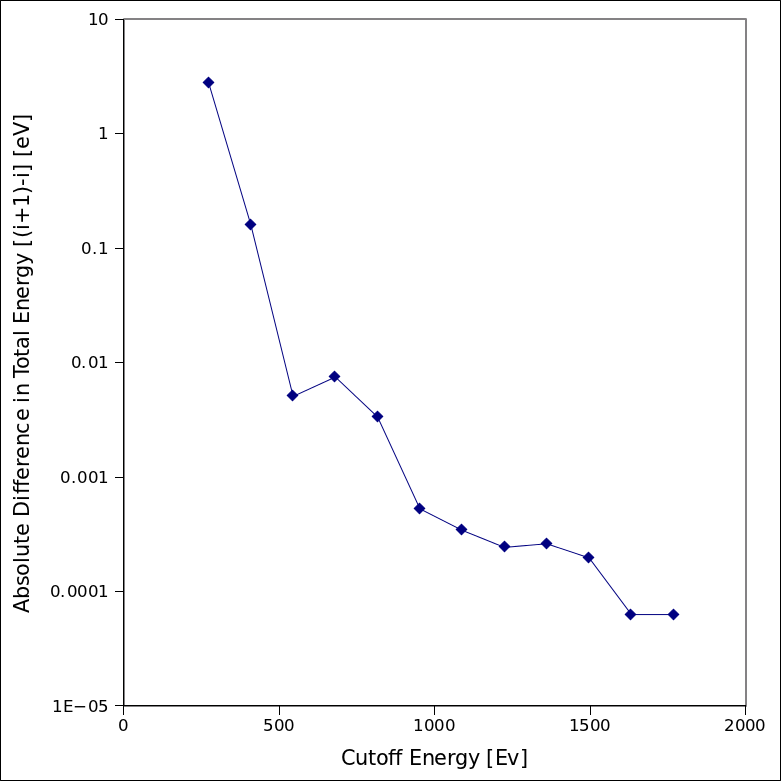
\includegraphics[totalheight=0.5\textheight]{ecut.png}
%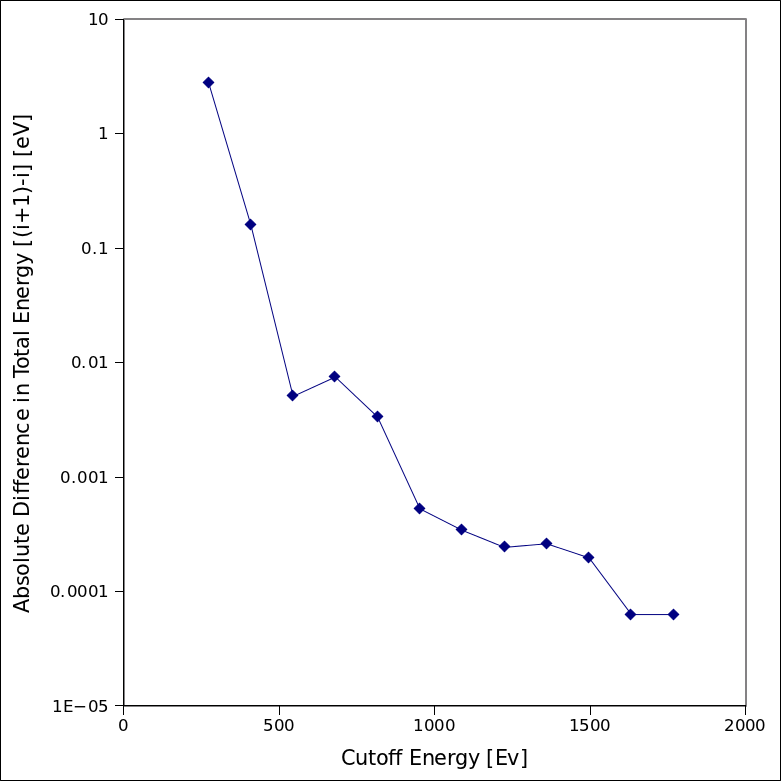
\includegraphics[scale=0.5]{ecut.png}
\caption{Convergence of Total Energy as a function of energy cutoff}
\label{fig:aNicePicture}
\end{figure}
\begin{center}
\begin{tabular}{|c|c|}
  \hline
  Energy Cutoff [Ry] & Time [CPU s] \\ \hline
 20  &   0.82   \\ \hline
 30  &   0.93	\\ \hline
 40  &   1.04 	\\ \hline
 50  &   1.13	\\ \hline
 60  &   1.21	\\ \hline
 70  &   1.89	\\ \hline
 80  &   2.06 	\\ \hline
 90  &   2.24	\\ \hline
 100 &   2.34  	\\ \hline
 110 &   2.54	\\ \hline
 120 &   2.91	\\ \hline
 130 &   3.08	\\ \hline
 140 &   3.24   \\ \hline     
\end{tabular}
\end{center}
\section*{Convergence w.r.t k-grid cutoff}

\begin{center}
\begin{tabular}{|c|c|}
  \hline
  K-point grid (nxnxn) & Number of Unique K-points \\ \hline
 1  &   1   \\ \hline
 2  &   3	\\ \hline
 4  &   8 	\\ \hline
 6  &   16	\\ \hline
 8  &   29	\\ \hline
 10  &   47	\\ \hline
 12  &   72	\\ \hline
\end{tabular}
\end{center}
\begin{figure}[h!]
\centering
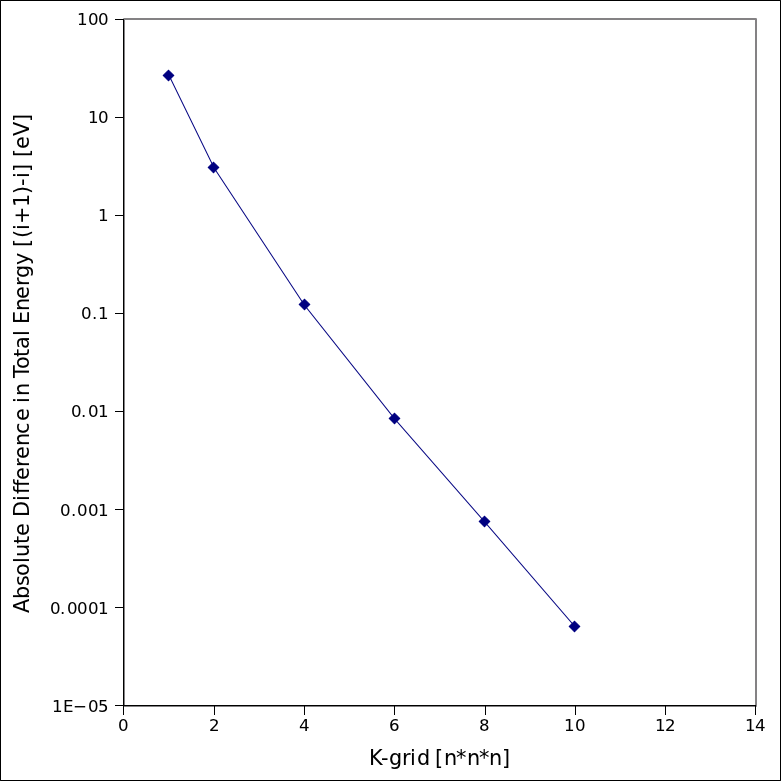
\includegraphics[totalheight=0.5\textheight]{kgrid.png}
%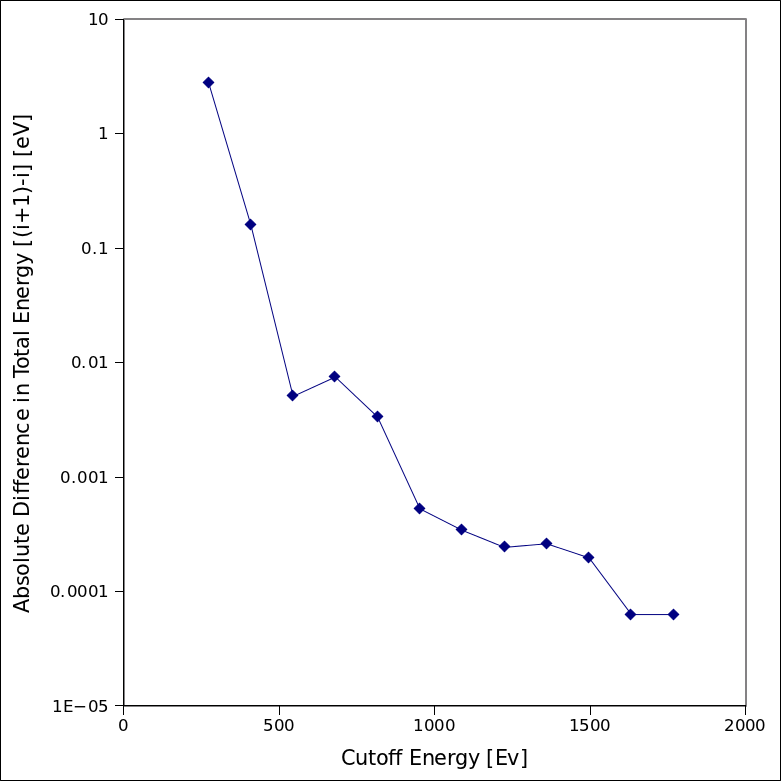
\includegraphics[scale=0.5]{ecut.png}
\caption{Convergence of Total Energy as a function of k-grid}
\label{fig:aNicePicture}
\end{figure}
\newpage
\section*{Convergence of forces w.r.t energy cutoff}
\begin{center}
\begin{tabular}{|c|c|}
  \hline
  Lattice Parameter & 6.74 [Bohr] \\ \hline
  Pseudopotential & C.pz-kjpaw.UPF \\ \hline
  K-grid & 4 x 4 x 4 Monkhorst-Pack  \\ \hline
  Unique K-points & 18  \\ \hline
\end{tabular}
\end{center}
\begin{figure}[h!]
\centering
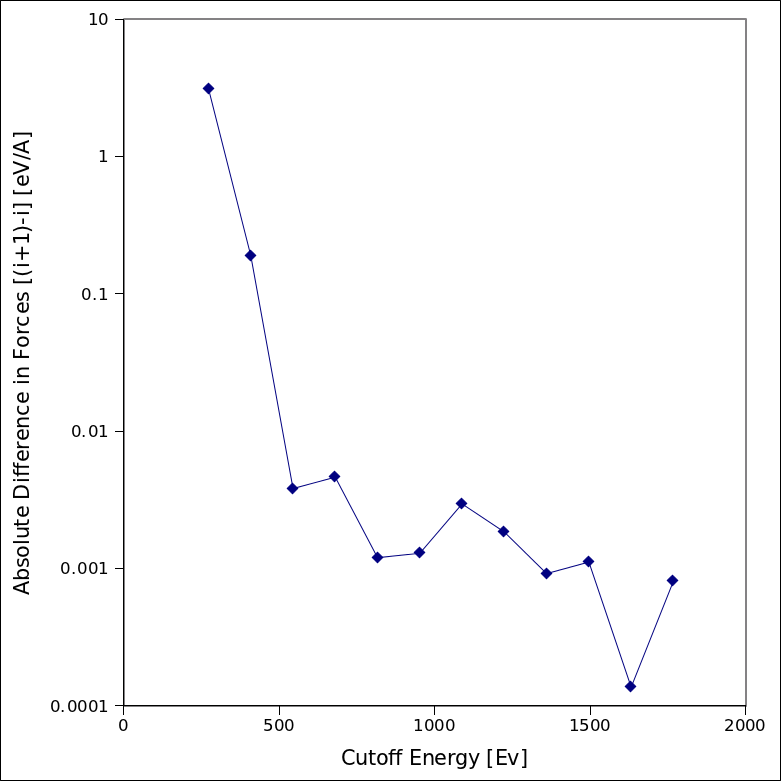
\includegraphics[totalheight=0.5\textheight]{forces.png}
%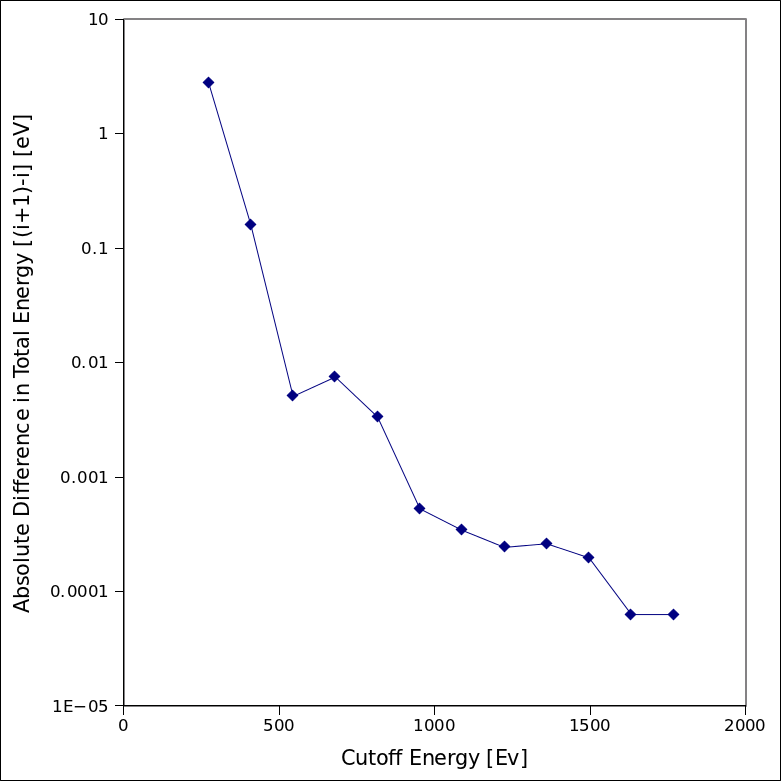
\includegraphics[scale=0.5]{ecut.png}
\caption{Convergence of Forces as a function of cutoff energy}
\label{fig:aNicePicture}
\end{figure}
\section*{Equilibrium Lattice Constant}
\begin{center}
\begin{tabular}{|c|c|}
  \hline
  Cutoff & 140 [Ry] \\ \hline
  K-grid & 8 x 8 x 8 Monkhorst-Pack  \\ \hline
  Unique K-points & 95 \\ \hline
\end{tabular}
\end{center}
\begin{figure}[h!]
\centering
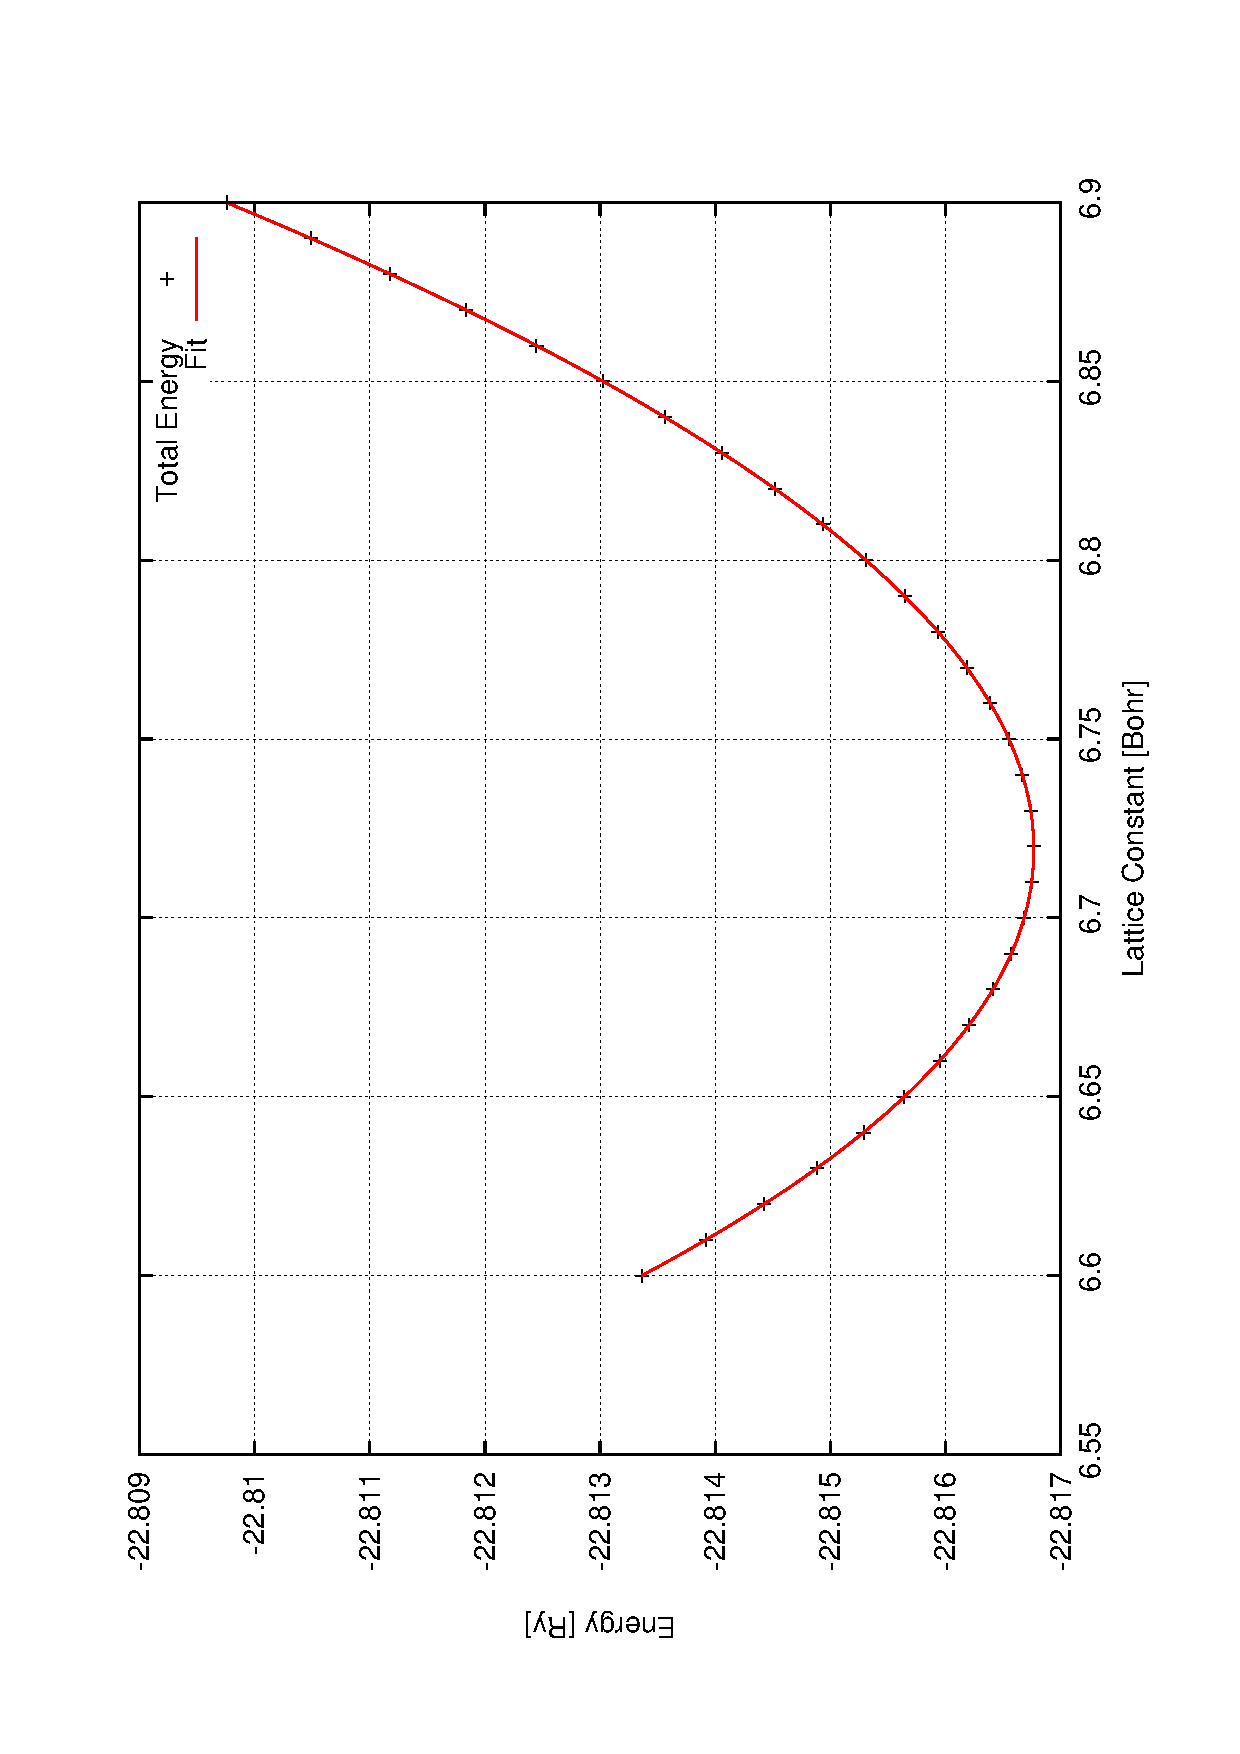
\includegraphics[totalheight=0.5\textheight, angle=-90]{bulk}
\caption{Total energy as a function of lattice constant}
\label{fig:aNicePicture}
\end{figure}
\begin{center}
\begin{tabular}{|c|c|c|}
  \hline
  Pseudopotential & Total Energy [Ry] & Calculated Bulk Modulus [Pa] \\ \hline
  C.pz-rrkjus.UPF & -22.8168   &   3.28E11  \\ \hline
  C.pz-kjpaw.UPF  & -35.5863   &   No fit \\ \hline
\end{tabular}
\end{center}
The calculated bulk modulus is on the same order of magnitude as experimental results of 4.42E11 [Pa].
\newpage
\section*{Script}
\begin{verbatim}
#!/bin/sh
############################################################################# 
LISTECUT='20 30 40 50 60 70 80 90 100 110 120 130 140' 

LISTKGRID='1 2 4 6 8 10 12'

LISTALAT='6.60 6.61 6.62 6.63 6.64 6.65 6.66 6.67 6.68 
6.69 6.70 6.71 6.72 6.73 6.74 6.75 6.76 6.77 6.78 6.79 
6.80 6.81 6.82 6.83 6.84 6.85 6.86 6.87 6.88 6.89 6.90'

PSEUDO_DIR="/home/sam/Documents/espresso-4.3.2/pseudo/"
SCRATCH="/home/sam/Documents/espresso-4.3.2/diac/scratch" 
OUTPUT="/home/sam/Documents/espresso-4.3.2/diac" 
EXEPATH="/home/sam/Documents/espresso-4.3.2/bin"

if [ ! -d $SCRATCH ]; then 
mkdir $SCRATCH 
fi 

if [ ! -d $PSEUDO_DIR ]; then 
mkdir $PSEUDO_DIR 
fi 

if [ ! -d $OUTPUT ]; then 
echo $MYDIR does not exist, please create it first 
exit 
 fi 
   
#for ecut in $LISTECUT 
#  do
#for kgrid in $LISTKGRID 
#  do 
for alat in $LISTALAT 
  do 
#rm -f $OUTPUT/diac.scf.$kgrid.in
#cat > $OUTPUT/diac.scf.$kgrid.in << EOF
#rm -f $OUTPUT/diac.scf.$ecut.in
#cat > $OUTPUT/diac.scf.$ecut.in << EOF
rm -f $OUTPUT/diac.scf.$alat.in
cat > $OUTPUT/diac.scf.$alat.in << EOF



  &control
    prefix='diamond',
    calculation='scf',
    outdir = '$SCRATCH' 
    pseudo_dir = '$PSEUDO_DIR' 
    tprnfor=.true.
 /
 &system    
    ibrav=  2, 
    !celldm(1) =6.74,
    celldm(1) =$alat, 
    nat=  2, ntyp= 1,
    !ecutwfc = $ecut,
    ecutwfc = 140,
 /
 &electrons
 /
ATOMIC_SPECIES
C  12.0107  C.pz-kjpaw.UPF
ATOMIC_POSITIONS
 C 0.00 0.00 0.05 
 C 0.25 0.25 0.25 
K_POINTS {automatic}
8 8 8 0 0 0
EOF

#$EXEPATH/pw.x < $OUTPUT/diac.scf.$ecut.in >  $OUTPUT/diac.scf.$ecut.out
#$EXEPATH/pw.x < $OUTPUT/diac.scf.$kgrid.in >  $OUTPUT/diac.scf.$kgrid.out
$EXEPATH/pw.x < $OUTPUT/diac.scf.$alat.in >  $OUTPUT/diac.scf.$alat.out
done

\end{verbatim}

\end{document}

